\section{Quantum Blackbox Algorithms}
\label{sec:blackbox}
The Fourier Transform is a powerful tool in most quantum algorithms for algebraic problems. Now that we have a structural handle on this tool, we use it to verify, generalize, and construct quantum algorithms.

In this section we first consider the structure of unitary oracles and then review the Deutsch-Jozsa, Grover's single shot, and hidden subgroup algorithms as examples of the approach.  These three initial algorithms were analyzed by Vicary in~\cite{vicary-tqa}, though the structure of the underlying oracles was assumed there.  We then expand on this base to develop a new quantum algorithm for the GROUPHOMID problem. The analysis of this algorithm is presented in Section~\ref{sec:grouphomid}.

\subsection{The abstract structure of unitary oracles}
\label{sec:unitaryoracles}

When we program an abstract problem into an oGCT, we have a choice of embeddings, but typically assign classical information to the classical states. This was, for example, the case in our treatment of the Fourier Transform. Of course, we will also want to consider how to program functions between those classical states. An equivalent definition for classical states is that they are self-conjugate comonoid homomorphisms from the trivial comonoid on the identity object to the classical structure monoid on a system. Classical functions will be self-conjugate comonoid homomorphisms in general.

\begin{defn}
\label{def:selfconj}
In a monoidal dagger-category, a comonoid homomorphism \\$f:\blackcomonoid{A} \to \graycomonoid{B}$ is \emph{self-conjugate} when the following property holds:
\begin{equation}
\label{eq:comonoidhomomorphismselfconjugate}
\begin{aligned}
\begin{tikzpicture}[xscale=1.4*\tikzxscale, yscale=1.4*\tikzyscale]
\node [morphism, wedge] (f) at (2,1) {$f$};
\draw (0,-1) to [out=up, in=left, in looseness=0.9] (1,2) node [graydot] {} to (1,2.5) node [graydot] {};
\draw (1,2) to [out=right, in=up] (f.north);
\draw (f.south) to [out=down, in=left] (3,0) node [blackdot] {} to [out=right, in=down, out looseness=0.9] (4,3);
\draw (3,0) to (3,-0.5) node [blackdot] {};
\node [graydot] at (1,2) {};
\end{tikzpicture}
\end{aligned}
\quad=\quad
\begin{aligned}
\begin{tikzpicture}[string]
\node (f) at (0,0) [morphism, wedge, hflip] {$f$};
\draw (0,-1.5) to (f.south);
\draw (f.north) to (0,1.5);
\end{tikzpicture}
\end{aligned}
\end{equation}
\end{defn}

\begin{lemma}
\label{lem:comonoidhomomorphismselfconjugate}
In {\bf Hilb}, comonoid homomorphisms $f:\blackcomonoid{A} \to \graycomonoid{B}$ of classical structures are self-conjugate.
\end{lemma}


\begin{proof}
Recall that comonoid homomorphisms between classical structures in \cat{Hilb} are exactly classical functions between the classical states~\cite{coecke2013new}. The linear maps on either side of~\eqref{eq:comonoidhomomorphismselfconjugate} will be the same if and only if their matrix elements are the same, obtained by composing with $\ket i$ at the bottom and $\bra j$ at the top. On the left-hand side, this gives the following result:
\begin{equation}
\begin{aligned}
\begin{tikzpicture}[xscale=1.4*\tikzxscale, yscale=1.4*\tikzyscale]
\node [morphism, wedge] (f) at (2,1) {$f$};
\draw (0,0) node [state] {$i$} to [out=up, in=left, in looseness=0.9] (1,2) node [graydot] {} to (1,2.5) node [graydot] {};
\draw (1,2) to [out=right, in=up] (f.north);
\draw (f.south)
    to [out=down, in=left] (3,0)
        node [blackdot] {}
    to [out=right, in=down, out looseness=0.9] (4,2)
        node [state, hflip] {$j$};
\draw (3,0) to (3,-0.5) node [blackdot] {};
\end{tikzpicture}
\end{aligned}
\quad=\quad
\begin{aligned}
\begin{tikzpicture}[xscale=1.4*\tikzxscale, yscale=1.4*\tikzyscale]
\node (f) [morphism, wedge] at (0,0) {$f$};
\draw (0,-0.75) node [state] {$j$} to (f.south);
\draw (0,0.75) node [state, hflip] {$i$} to (f.north);
\end{tikzpicture}
\end{aligned}
\quad=\quad
\left\{
\begin{array}{ll}
1 & \text{ if } i=f(j), \\
0 & \text{ if } i \neq f(j).
\end{array}
\right.
\end{equation}
On the right we can do this calculation:
\begin{equation}
\begin{aligned}
\begin{tikzpicture}[xscale=1.4*\tikzxscale, yscale=1.4*\tikzyscale]
\node (f) [morphism, wedge, hflip] at (0,0) {$f$};
\draw (0,-0.75) node [state] {$i$} to (f.south);
\draw (0,0.75) node [state, hflip] {$j$} to (f.north);
\end{tikzpicture}
\end{aligned}
\quad=\quad
\left(
\begin{aligned}
\begin{tikzpicture}[xscale=1.4*\tikzxscale, yscale=1.4*\tikzyscale]
\node (f) [morphism, wedge] at (0,0) {$f$};
\draw (0,-0.75) node [state] {$j$} to (f.south);
\draw (0,0.75) node [state, hflip] {$i$} to (f.north);
\end{tikzpicture}
\end{aligned}
\right) ^\dagger
\quad=\quad
\left\{
\begin{array}{ll}
1 & \text{ if } i=f(j) \\
0 & \text{ if } i \neq f(j)
\end{array}
\right\}^\dagger 
\quad = \quad
\left\{
\begin{array}{ll}
1 & \text{ if } i=f(j), \\
0 & \text{ if } i \neq f(j).
\end{array}
\right.
\end{equation}
This is the same result as for the left-hand side, and so Equation~\eqref{eq:comonoidhomomorphismselfconjugate} holds.
\end{proof}

The oracle that we will build here is similar to the CNOT from Section~\ref{ex:cnot}. Recall that a pair of symmetric dagger-Frobenius algebras can be used to build a linear map in the following way:
\begin{equation}
\sqrt{\ud(A)}\,\,
\begin{pic}[xscale=\tikzxscale, yscale=\tikzyscale]
\node (b) [graydot] at (0,0) {};
\node (w) [whitedot] at (1,1) {};
\draw (-0.75,2) to [out=down, in=left] (b.center);
\draw (b.center) to [out=right, in=left] (w.center);
\draw (w.center) to (1,2);
\draw (b.center) to (0,-1);
\draw (w.center) to [out=right, in=up] (1.75,-1);
\end{pic}
\end{equation}
Here we have assumed that we operate in a category where square roots of scalars exist.  The two algebras are complementary exactly when this composite is unitary, as we show in the following theorem.

\begin{theorem}[Complementarity via a unitary]
\label{thm:complementarityunitary}
  In a dagger symmetric monoidal category, two symmetric dagger-Frobenius algebras are complementary if and only if the composite~\eqref{eq:generalizedcnot} is unitary.
\end{theorem}
\begin{proof}
  Composing ~\eqref{eq:generalizedcnot} with its adjoint in one order, we obtain the following:
\begin{equation}
\label{eq:generalizedcnotunitaryproof}
\begin{aligned}
  \begin{tikzpicture}[xscale=1.4*\tikzxscale, yscale=1.4*\tikzyscale]
  \node at (-1.6,-2.6) {$\ud (A)$};
  \node (A) at (0,0) {};
  \node (B) at (1.75,0) {};
  \node (b1) [graydot] at (0,-1) {};
  \node (w1) [whitedot] at (1,-2) {};
  \node (w2) [whitedot] at (1,-3) {};
  \node (b2) [graydot] at (0,-4) {};
  \node (C) at (0,-5) {};
  \node (D) at (1.75,-5) {};
  \draw (A.center) to (b1.center);
  \draw (b1.center) to [out=right, in=left] (w1.center);
  \draw (w1.center) to (w2.center);
  \draw (w2.center) to [out=left, in=right] (b2.center);
  \draw (b2.center) to (C.center);
  \draw (w2.center) to [out=right, in=up] (D.center);
  \draw (w1.center) to [out=right, in=down] (B.center);
  \draw (b1.center) to [out=left, in=left] (b2.center);
  \end{tikzpicture}
  \end{aligned}
  \stackrel{\mbox{\small Thm}~\ref{thm:spider}}{=}
  \begin{aligned}
  \begin{tikzpicture}[xscale=1.4*\tikzxscale, yscale=1.4*\tikzyscale]
  \node at (-2.1,-2.6) {$\ud (A)$};
  \node (A) at (-1.75,0) {};
  \node (B) at (0.5,0) {};
  \node (w1) [whitedot] at (0.5,-1.0) {};
  \node (w2) [whitedot] at (1.25,-3) {};
  \node (w3) [whitedot] at (0,-2) {};
  \node (b1) [graydot] at (-1,-2) {};
  \node (b2) [graydot] at (0,-4) {};
  \node (b3) [graydot] at (-0.5,-1) {};
  \node (C) at (0,-5) {};
  \node (D) at (2,-5) {};
  \draw (A.center) to [out=down, in=left] (b1.center);
  \draw (w1.center) to [out=right, in=up] (w2.center);
  \draw (w2.center) to [out=left, in=right] (b2.center);
  \draw (b2.center) to (C.center);
  \draw (w2.center) to [out=right, in=up] (D.center);
  \draw (w1.center) to [out=up, in=down] (B.center);
  \draw (b1.center) to [out=down, in=left] (b2.center);
  \draw (b1.center) to [out=right, in=left] (b3.center);
  \draw (b3.center) to [out=right, in=left] (w3.center);
  \draw (w3.center) to [out=right, in=left] (w1.center);
  \end{tikzpicture}
  \end{aligned}
  \stackrel{\eqref{eq:monoid}}{=}
  \begin{aligned}
  \begin{tikzpicture}[xscale=1.4*\tikzxscale, yscale=1.4*\tikzyscale]
  \node at (-2,-3.1) {$\ud (A)$};  
  \node (A) at (-1,0) {};
  \node (B) at (1.5,0) {};
  \node (w1) [whitedot] at (1.5,-1.0) {};
  \node (w2) [whitedot] at (1.0,-2) {};
  \node (w3) [whitedot] at (0.5,-3) {};
  \node (b1) [graydot] at (0.5,-4) {};
  \node (b2) [graydot] at (0,-5) {};
  \node (b3) [graydot] at (0,-2) {};
  \node (C) at (0,-6) {};
  \node (D) at (2.5,-6) {};
  \draw (A.center) to [out=down, in=left, in looseness=0.6] (b2.center);
  \draw (w1.center) to [out=left, in=up] (w2.center);
  \draw (w2.center) to [out=right, in=right] (b1.center);
  \draw (b2.center) to (C.center);
  \draw (w1.center) to [out=right, in=up, out looseness=0.6] (D.center);
  \draw (w1.center) to [out=up, in=down] (B.center);
  \draw (b1.center) to [out=down, in=right] (b2.center);
  \draw (b1.center) to [out=left, in=left] (b3.center);
  \draw (b3.center) to [out=right, in=left] (w3.center);
  \draw (w2.center) to [out=left, in=right] (w3.center);
  \end{tikzpicture}
  \end{aligned}  

\end{equation}
  If the complementarity condition~\eqref{eq:complementarity} holds then this is clearly the identity on \mbox{$A \otimes A$}. The other composite can be shown to be the identity in a similar way, and so~\eqref{eq:generalizedcnot} is unitary.

  Conversely, suppose~\eqref{eq:generalizedcnot} is unitary. Then the final expression of~\eqref{eq:generalizedcnotunitaryproof} certainly equals the identity on $A \otimes A$:
\begin{equation}
\begin{aligned}
\begin{tikzpicture}[xscale=1.4*\tikzxscale, yscale=1.1*\tikzyscale]
  \draw (0.5,-5) to (0.5,1);
  \draw (-1.5,-5) to (-1.5,1);
\end{tikzpicture}
\end{aligned}
\quad=\quad
\begin{aligned}
\begin{tikzpicture}[xscale=1.4*\tikzxscale, yscale=1.1*\tikzyscale]
  \node at (-1.9,-3.1) {$\ud (A)$};  
  \node (A) at (-1,0) {};
  \node (B) at (1.5,0) {};
  \node (w1) [whitedot] at (1.5,-1.0) {};
  \node (w2) [whitedot] at (1.0,-2) {};
  \node (w3) [whitedot] at (0.5,-3) {};
  \node (b1) [graydot] at (0.5,-4) {};
  \node (b2) [graydot] at (0,-5) {};
  \node (b3) [graydot] at (0,-2) {};
  \node (C) at (0,-6) {};
  \node (D) at (2.5,-6) {};
  \draw (A.center) to [out=down, in=left, in looseness=0.6] (b2.center);
  \draw (w1.center) to [out=left, in=up] (w2.center);
  \draw (w2.center) to [out=right, in=right] (b1.center);
  \draw (b2.center) to (C.center);
  \draw (w1.center) to [out=right, in=up, out looseness=0.6] (D.center);
  \draw (w1.center) to [out=up, in=down] (B.center);
  \draw (b1.center) to [out=down, in=right] (b2.center);
  \draw (b1.center) to [out=left, in=left] (b3.center);
  \draw (b3.center) to [out=right, in=left] (w3.center);
  \draw (w2.center) to [out=left, in=right] (w3.center);
\end{tikzpicture}
\end{aligned}

\end{equation}
 Composing with the black counit at the top-left and the white unit at the bottom-right then gives back complementarity condition~\eqref{eq:complementarity} as required:
\begin{equation}
  \begin{aligned}
  \begin{tikzpicture}[xscale=1.4*\tikzxscale, yscale=1.1*\tikzyscale]
  \node (w) [whitedot] at (-0.5,-4) {};
  \node (b) [graydot] at (-1.5,0) {}; 
  \draw (-0.5,-4) to (-0.5,1);
  \draw (-1.5,-5) to (-1.5,0);
  \end{tikzpicture}
  \end{aligned}
  \,\,\,\,= 
  \begin{aligned}
  \begin{tikzpicture}[xscale=1.4*\tikzxscale, yscale=1.1*\tikzyscale]
  \node at (-1.9,-3.1) {$\ud (A)$}; 
  \node (w) [graydot] at (-1,0) {};
  \node (b) [whitedot] at (2.5,-6) {}; 
  \node (A) at (-1,0) {};
  \node (B) at (1.5,0) {};
  \node (w1) [whitedot] at (1.5,-1.0) {};
  \node (w2) [whitedot] at (1.0,-2) {};
  \node (w3) [whitedot] at (0.5,-3) {};
  \node (b1) [graydot] at (0.5,-4) {};
  \node (b2) [graydot] at (0,-5) {};
  \node (b3) [graydot] at (0,-2) {};
  \node (C) at (0,-6) {};
  \node (D) at (2.5,-6) {};
  \draw (A.center) to [out=down, in=left, in looseness=0.6] (b2.center);
  \draw (w1.center) to [out=left, in=up] (w2.center);
  \draw (w2.center) to [out=right, in=right] (b1.center);
  \draw (b2.center) to (C.center);
  \draw (w1.center) to [out=right, in=up, out looseness=0.6] (D.center);
  \draw (w1.center) to [out=up, in=down] (B.center);
  \draw (b1.center) to [out=down, in=right] (b2.center);
  \draw (b1.center) to [out=left, in=left] (b3.center);
  \draw (b3.center) to [out=right, in=left] (w3.center);
  \draw (w2.center) to [out=left, in=right] (w3.center);
  \end{tikzpicture}
  \end{aligned}
  \,\,= \,\,  \mathrm{d}(A) \;
  \begin{pic}[xscale=1.4*\tikzxscale, yscale=1.4*\tikzyscale]
\draw (-0.5,0.25) to (-0.5,1) node [graydot] {} to [out=left, in=right] (-1,2) node [graydot] {} to [out=left, in=right] (-1.5,1.5) node [whitedot] {} to [out=left, in=down] (-2,2) to [out=up, in=left] (-0.75,3) node (a) [whitedot] {} to [out=right, in=right] (-0.5,1);
\draw (a.center) to +(0,0.75);
\end{pic}

\end{equation}
This completes the proof.
\end{proof}

This pair of complementary observables automatically gives rise to a much larger family of unitaries, one for each self-conjugate comonoid homomorphism onto one of the classical structures in the pair. Lemma~\ref{lem:comonoidhomomorphismselfconjugate} demonstrated that in \cat{FHilb}, every comonoid homomorphism of classical structures is self-conjugate.
\begin{defn}[Oracle]
\label{oracle}
In a symmetric monoidal dagger-category, given a dagger-Frobenius comonoid $\blackcomonoid{A}$, a pair of complementary symmetric dagger-Frobenius comonoids \graycomonoid{B} and \whitecomonoid{B}, and a self-conjugate comonoid homomorphism $f : \blackcomonoid{A} \to \graycomonoid{B}$, the \emph{oracle} is defined to be the following endomorphism of $A \otimes B$:
\begin{equation}
\label{eq:oracle}
\sqrt{\ud(A)}
\begin{pic}[xscale=1.8*\tikzxscale, yscale=1.3*\tikzyscale]
    \node (dot) [blackdot] at (0,1) {};
    \node (f) [morphism, wedge] at (0.7,2) {$f$};
    \node (m) [whitedot] at (1.4,3) {};
\draw (0,0.25)
        node [below] {$A$}
    to (0,1)
    to [out=left, in=south] (-0.7,2)
    to (-0.7,3.75)
        node [above] {$A$};
\draw (0,1)
    to [out=right, in=south] (f.south);
\draw  (f.north)
    to [out=up, in=left] (1.4,3)
    to [out=right, in=up] +(0.7,-1)
    to (2.1,0.25)
        node [below] {$B$};;
\draw (m.center) to +(0,0.75) node [above] {$B$};
\end{pic}

\end{equation}
\end{defn}

\begin{theorem}
\label{thm:familyofunitaries}
Oracles are unitary.
\end{theorem}
\begin{proof}
To demonstrate that the oracle~\eqref{eq:oracle} is unitary, we must compose it with its adjoint on both sides and show that we get the identity in each case. In one case, we obtain the following, making use of the Frobenius laws, self-conjugacy of $f$, associativity and coassociativity, the fact that $f$ preserves comultiplication, the complementarity condition, the fact that $f$ preserves the counit, and the unit and counit laws:
\begin{align*}
&\ud(A)
\begin{aligned}
\begin{tikzpicture}[xscale=2*\tikzxscale, yscale=1.2*\tikzyscale]
\node (A) at (0,2) {};
\node (B) at (1.75,0) {};
\node (b1) [blackdot] at (0,1) {};
\node (w1) [whitedot] at (1,-1) {};
\node (w2) [whitedot] at (1,-2) {};
\node (b2) [blackdot] at (0,-4) {};
\node (C) at (0,-5) {};
\node (D) at (1.75,-5) {};
\node (f1) [morphism, wedge] at (0.5,-3) {$f$};
\node (f2) [morphism, wedge, hflip] at (0.5,0) {$f$};
\draw (A.center) to (b1.center);
\draw (b1.center) to [out=right, in=up] (f2.north);
\draw (f2.south) to [out=down, in=left] (w1.center);
\draw (w1.center) to (w2.center);
\draw (w2.center) to [out=left, in=up] (f1.north);
\draw (b2.center) to (C.center);
\draw (w2.center) to [out=right, in=up] (1.5,-3 |- f1.north) to (1.5,-5);
\draw (w1.center) to [out=right, in=down] (1.5,1 |- f2.south) to (1.5,2);
\draw (b1.center) to [out=left, in=up] (-0.5,0 |- f2.north) to (-0.5,0 |- f1.south) to [out=down, in=left] (b2.center);
\draw (f1.south) to [out=down, in=right] (b2.center);
\end{tikzpicture}
\end{aligned}
=\,\,
\ud(A)
\hspace{-3pt}
\begin{aligned}
\begin{tikzpicture}[xscale=2.3*\tikzxscale, yscale=1.4*\tikzyscale]
\node (f1) [morphism, wedge] at (0.5,-4) {$f$};
\node (f2) [morphism, wedge, hflip] at (-0.5,-2) {$f$};
\node (A) at (-2,0) {};
\node (B) at (0.5,0) {};
\node (w1) [whitedot] at (0.5,-2.0) {};
\node (w2) [whitedot] at (1.0,-3) {};
\node (w3) [whitedot] at (-0.125,-3) {};
\node (b1) [blackdot] at (-1.5,-3) {};
\node (b2) [blackdot] at (0,-5) {};
\node (b3) [blackdot] at (-0.75,-1) {};
\node (C) at (0,-6) {};
\node (D) at (1.5,-6) {};
\draw (A.center) to +(0,-1.5) to [out=down, in=left] (b1.center);
\draw (w1.center) to [out=right, in=up] (w2.center);
\draw (w2.center) to [out=left, in=up] (f1.north);
\draw (f1.south) to [out=down, in=right] (b2.center);
\draw (b2.center) to (C.center);
\draw (w2.center) to [out=right, in=up] (D.center |- f1.north) to (D.center);
\draw (w1.center) to [out=up, in=down] (B.center);
\draw (b1.center) to [out=down, in=left] (b2.center);
\draw (b1.center) to [out=right, in=left] (b3.center);
\draw (f2.south) to [out=down, in=left] (w3.center);
\draw (w3.center) to [out=right, in=left] (w1.center);
\draw (b3.center) to [out=right, in=up] (f2.north);
\end{tikzpicture}
\end{aligned}
=\,\,
\ud(A)
\hspace{-3pt}
\begin{aligned}
\begin{tikzpicture}[xscale=2.3*\tikzxscale, yscale=1.4*\tikzyscale]
\node (f1) [morphism, wedge] at (0.5,-4) {$f$};
\node (f2) [morphism, wedge] at (-1,-2) {$f$};
\node (A) at (-2,0) {};
\node (B) at (0.68,0) {};
\node (w1) [whitedot] at (0.68,-2.0) {};
\node (w2) [whitedot] at (1.0,-3) {};
\node (w3) [whitedot] at (0.25,-3) {};
\node (b1) [blackdot] at (-1.5,-3) {};
\node (b2) [blackdot] at (0,-5) {};
\node (b3) [graydot] at (-0.5,-1) {};
\node (C) at (0,-6) {};
\node (D) at (1.5,-6) {};
\draw (A.center) to +(0,-1.5) to [out=down, in=left] (b1.center);
\draw (w1.center) to [out=right, in=up] (w2.center);
\draw (w2.center) to [out=left, in=up] (f1.north);
\draw (f1.south) to [out=down, in=right] (b2.center);
\draw (b2.center) to (C.center);
\draw (w2.center) to [out=right, in=up] (D.center |- f1.north) to (D.center);
\draw (w1.center) to [out=up, in=down] (B.center);
\draw (b1.center) to [out=down, in=left] (b2.center);
\draw (w3.center) to [out=left, in=right] (b3.center);
\draw (f2.south) to [out=down, in=right] (b1.center);
\draw (w3.center) to [out=right, in=left] (w1.center);
\draw (b3.center) to [out=left, in=up] (f2.north);
\end{tikzpicture}
\end{aligned}
\\
&
\hspace{2cm}
= \,\,\ud(A)
\begin{aligned}
\begin{tikzpicture}[xscale=2.6*\tikzxscale, yscale=1.4*\tikzyscale]
\node (f1) [morphism, wedge] at (-0.25,-3) {$f$};
\node (f2) [morphism, wedge] at (1.25,-3) {$f$};
\node (A) at (-1,0) {};
\node (B) at (1.5,0) {};
\node (w1) [whitedot] at (1.5,-1.0) {};
\node (w2) [whitedot] at (1.0,-2) {};
\node (w3) [whitedot] at (0.5,-2.5) {};
\node (b1) [blackdot] at (0.5,-4) {};
\node (b2) [blackdot] at (0,-5) {};
\node (b3) [graydot] at (0,-2) {};
\node (C) at (0,-6) {};
\node (D) at (2.25,-6) {};
\draw (A.center) to [out=down, in=left, in looseness=0.59] (b2.center);
\draw (w1.center) to [out=left, in=up] (w2.center);
\draw (w2.center) to [out=right, in=up] (f2.north);
\draw (b2.center) to (C.center);
\draw (w1.center) to [out=right, in=up, out looseness=0.45] (D.center);
\draw (w1.center) to [out=up, in=down] (B.center);
\draw (b1.center) to [out=down, in=right] (b2.center);
\draw (b1.center) to [out=left, in=down] (f1.south);
\draw (b3.center) to [out=right, in=left] (w3.center);
\draw (w2.center) to [out=left, in=right] (w3.center);
\draw (f1.north) to [out=up, in=left] (b3.center);
\draw (f2.south) to [out=down, in=right] (b1.center);
\end{tikzpicture}
\end{aligned}
= \,\,\ud(A)
\begin{aligned}
\begin{tikzpicture}[xscale=2.6*\tikzxscale, yscale=1.4*\tikzyscale]
\node (f) [morphism, wedge] at (0.5,-4) {$f$};
\node (A) at (-0.5,0) {};
\node (B) at (1.5,0) {};
\node (w1) [whitedot] at (1.5,-1.0) {};
\node (w2) [whitedot] at (1.0,-2) {};
\node (w3) [whitedot] at (0.5,-2.5) {};
\node (b1) [graydot] at (0.5,-3.25) {};
\node (b2) [blackdot] at (0,-5) {};
\node (b3) [graydot] at (0,-2) {};
\node (C) at (0,-6) {};
\node (D) at (2,-6) {};
\draw (A.center) to +(0,-4) to [out=down, in=left] (b2.center);
\draw (w1.center) to [out=left, in=up] (w2.center);
\draw (w2.center) to [out=right, in=right] (b1.center);
\draw (b2.center) to (C.center);
\draw  (D.center) to +(0,4) to [out=up, in=right] (w1.center);
\draw (w1.center) to [out=up, in=down] (B.center);
\draw (b1.center) to [out=down, in=up] (f.north);
\draw (f.south) to [out=down, in=right] (b2.center);
\draw (b1.center) to [out=left, in=left] (b3.center);
\draw (b3.center) to [out=right, in=left] (w3.center);
\draw (w2.center) to [out=left, in=right] (w3.center);
\end{tikzpicture}
\end{aligned}
\\
&
\hspace{2cm}
=\hspace{5pt}
\begin{aligned}
\begin{tikzpicture}[xscale=2.6*\tikzxscale, yscale=1.2*\tikzyscale]
\node (f) [morphism, wedge] at (0.5,-4) {$f$};
\node (A) at (-0.5,0) {};
\node (B) at (1.5,0) {};
\node (w1) [whitedot] at (1.5,-1.0) {};
\node (w2) [whitedot] at (1.0,-2) {};
\node (b1) [graydot] at (0.5,-3) {};
\node (b2) [blackdot] at (0,-5) {};
\node (C) at (0,-6) {};
\node (D) at (2,-6) {};
\draw (A.center) to +(0,-4) to [out=down, in=left] (b2.center);
\draw (w1.center) to [out=left, in=up] (w2.center);
\draw (b2.center) to (C.center);
\draw  (D.center) to +(0,4) to [out=up, in=right] (w1.center);
\draw (w1.center) to [out=up, in=down] (B.center);
\draw (b1.center) to [out=down, in=up] (f.north);
\draw (f.south) to [out=down, in=right] (b2.center);
\end{tikzpicture}
\end{aligned}
\hspace{5pt}=\hspace{5pt}
\begin{aligned}
\begin{tikzpicture}[xscale=2.6*\tikzxscale, yscale=1.2*\tikzyscale]
\node (A) at (-0.5,0) {};
\node (B) at (1.5,0) {};
\node (w1) [whitedot] at (1.5,-1.0) {};
\node (w2) [whitedot] at (1.0,-2) {};
\node (b1) [blackdot] at (0.5,-4) {};
\node (b2) [blackdot] at (0,-5) {};
\node (C) at (0,-6) {};
\node (D) at (2,-6) {};
\draw (A.center) to +(0,-4) to [out=down, in=left] (b2.center);
\draw (w1.center) to [out=left, in=up] (w2.center);
\draw (b2.center) to (C.center);
\draw  (D.center) to +(0,4) to [out=up, in=right] (w1.center);
\draw (w1.center) to [out=up, in=down] (B.center);
\draw (b1.center) to [out=down, in=right] (b2.center);
\end{tikzpicture}
\end{aligned}
\hspace{5pt}=\hspace{5pt}
\begin{aligned}
\begin{tikzpicture}[xscale=2*\tikzxscale, yscale=1.2*\tikzyscale]
\draw (0,0) to (0,6);
\draw (1.5,0) to (1.5,6);
\end{tikzpicture}
\end{aligned}
\end{align*}
There is a similar argument that the other composite also gives the identity. \end{proof}

Note that this construction works for pairs of observables that a complementary, but not necessarily strongly complementary.  Still, in the examples we consider, we will use strongly complementary $(\dotonly{graydot},\dotonly{whitedot})$ as we wish to embed an internal group onto them.

\subsection{The Deutsch-Jozsa algorithm}
In this section, the abstract structure of the Deutsch-Jozsa (DJ) quantum algorithm is presented and its function is verified abstractly, following~\cite{vicary-tqa}. We recall that the Deutsch-Jozsa algorithm presents a quantum algorithm with an exponential speedup over exact classical computation~\cite{deutsch1992rapid}.  In its original formulation, given a function $f:\{0,1\}^n\to\{0,1\}$ that is promised to be either constant or balanced (i.e. outputs the same number of 0's as 1's), the algorithm determines which of the two classes $f$ is in. As we will see this formulation can be easily verified and generalized by the oGCT approach.

First we define the promise at the level of processes in an oGCT.

\begin{defn}
Let $A$ and $B$ be systems in an oGCT such that $A$ has an internal group $(\mathbb{G},\dotonly{altwhitedot},\dotonly{blackdot})$ and $B$ has an internal group $(\mathbb{H},\dotonly{graydot},\dotonly{whitedot})$. A process $f:A\to B$ is
\begin{itemize}
\item[(i)] \emph{constant} when for \dotonly{whitedot}-classical state $c:I\to B $
\begin{equation}
\begin{aligned}
\begin{tikzpicture}[yscale=1]
\node (f) [morphism, wedge, scale=1] at (0,0) {$f$};
\draw (0,-1) to (f.south);
\draw (f.north) to (0,1);
\end{tikzpicture}
\end{aligned}
\;=
\begin{aligned}
\begin{tikzpicture}[yscale=1]
\draw (0,-1) to (0,-.4)
    node [blackdot] {};
\draw (0,0.5) node [state, scale=1] {$c$} to (0,1);
\end{tikzpicture}
\end{aligned}
\end{equation}
\item[(ii)] \emph{balanced} when for non-trivial representation $\sigma:B\to I$
\begin{equation}
\begin{aligned}
\begin{tikzpicture}[string, yscale=1]
\node [morphism, wedge, scale=1] (f) at (0,0) {$f$};
\draw (0,-0.85) node [blackdot] {} to (f.south);
\node [morphism, wedge, scale=1] at (0,1){$\sigma$};
\draw (f.north) to (0,0.65) ;
\end{tikzpicture}
\end{aligned}
\;=\;
0
\end{equation} 
\end{defn}

It is easy to see that this definition coincides with the original formulation in $\cat{FHilb}$ for internal groups $\mathbb{G}=\mathbb{Z}_2^n$ and $\mathbb{H}=\mathbb{Z}_2$. In this case the \dotonly{whitedot}-classical states of $B$ are the group elements $\{0,1\}$, so a constant function simply ignores all input (as \tinycounit[blackdot] send all input to 1)  and outputs one element. In the balanced case, there is only one non-trivial representation of $\mathbb{Z}_2$, namely $\sigma(0)=1$ and $\sigma(1)=-1$. Thus
\begin{align}
\sigma\circ f\circ\tinyunit[blackdot] = \sigma \left(\sum_{x\in\mathbb{H}}\ket{f(x)}\right) = \sum_{x\in\mathbb{H}}\sigma\left(\ket{f(x)}\right),
\end{align}
which is clearly 0 if and only if half the number of inputs for which $f(x)=0$ is the same as the number of inputs for which $f(x)=1$. Picking different internal groups and representations gives different behaviors for balanced functions.

\begin{example}
Let $\mathbb{G}=\mathbb{Z}_2^n$ and $\mathbb{H}=\mathbb{Z}_2\times\mathbb{Z}_2$. We then have a choice of different non-trivial representations. Choose $\sigma = (1,-1,1,-1)$. Denoting $\#f_0$ as the number of inputs for which $f(x) = 0$, balanced functions are now $f$ such that:
\begin{align*}
\#f_{00}+\#f_{10} = \#f_{01}+\#f_{11}
\end{align*}
\end{example}

Directly mapping the (rotated) quantum circuit for the DJ algorithm into an oGCT process gives the following, where the internal groups $(\mathbb{G},\dotonly{altwhitedot},\dotonly{blackdot})$ and $(\mathbb{H},\dotonly{graydot},\dotonly{whitedot})$ are inherited from the promise of constant and balanced:
\begin{align}
\begin{aligned}
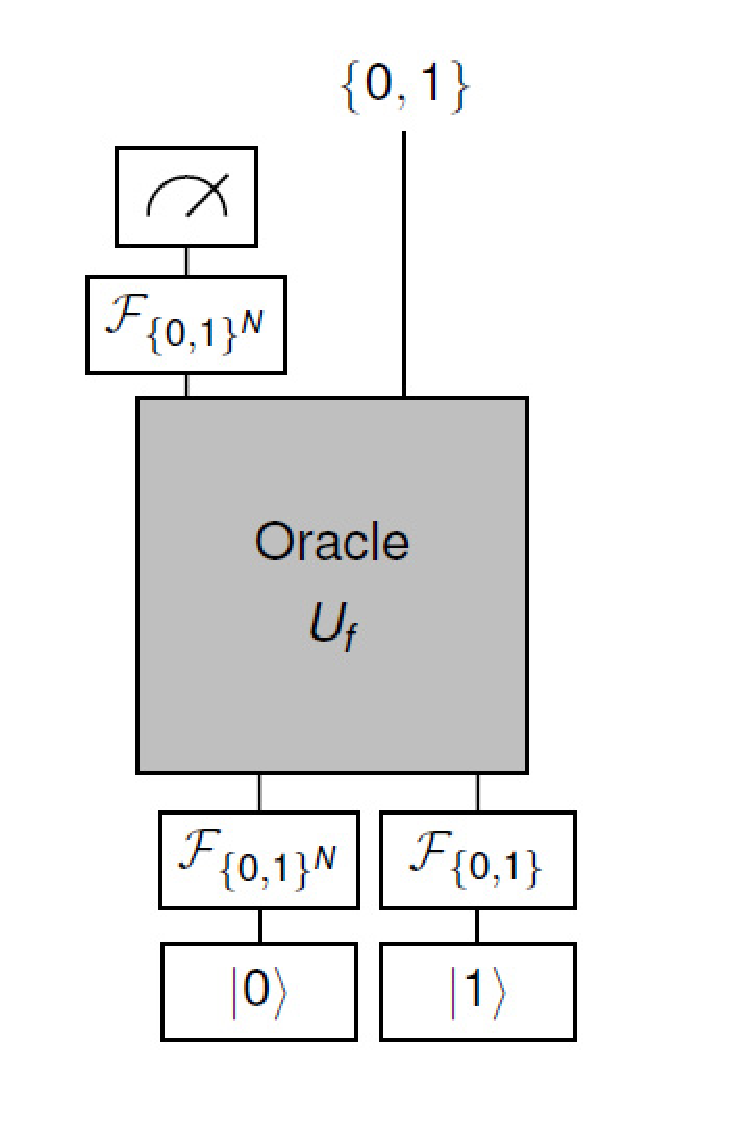
\includegraphics[width=14em]{images/DJQcircuit.eps}
\end{aligned}
\mapsto
\qquad
\begin{aligned}
\begin{tikzpicture}[thick, scale=0.75]
\draw [thick, white] (-1.33,6) rectangle (2.975,1);
    \node (dot) [blackdot] at (0,1) {};
    \node (f) [morphism, wedge, width=8pt, anchor=south, thick, node on layer=foreground] at (0.7,2) {$f$};
    \node (m) [whitedot] at ([xshift=0.7cm, yshift=1cm] f.north) {};
    \node (ftl) [morphism] at ([yshift=1.5cm] m.center -| -0.7,1) {$\mathcal{F}$};
    \node (ftb) [morphism] at (0,-0.25) {$\mathcal{F}$};
    \node (ftr) [morphism] at (2.1,-0.25) {$\mathcal{F}$};    
    \node (dd) [altwhitedot] at ([yshift=2.5cm] m.center -| -0.7,1) {};
    \draw [use as bounding box, draw=none] (-2,-2) rectangle +(6,10);
\draw (0,-1.5)
        node [altwhitedot] (bdot) {}
    to (ftb.south);       
\draw (ftb.north) to (0,1)
    to [out=\nwangle, in=south] (-0.7,2)
    to (ftl.south);
\draw (ftl.north) to (dd.south);
\draw (0,1)
    to [out=\neangle, in=south] (f.south);
\draw  (f.north)
    to [out=up, in=\swangle] +(0.7,1)
    to [out=\seangle, in=up] +(0.7,-1)
    to (ftr.north);
\draw (ftr.south)    
    to (2.1,-1.5)
        node [whitedot] (sigmadag) {$\pi$};
\draw (m.center) to (1.4,6.75)
        node [above] {$\{0,1\}$};
\node at ([xshift=-14, yshift=38pt] f.center) {\small Oracle};        
%\node [anchor=east] at ([xshift=3pt] bdot.west) {$\scriptstyle \frac{1}{\sqrt{|S|}}$};
%\node [anchor=east] at ([xshift=0pt] dd.west) {$\scriptstyle \frac{1}{\sqrt{|S|}}$};
%\node [anchor=east] at ([xshift=2pt] sigmadag.west) {$\scriptstyle \frac{1}{\sqrt{2}}$};
\node [draw, dotted, minimum width=2.8cm, minimum height=2.7cm, thick] at ([yshift=2pt] f.center) {};
\end{tikzpicture}
\end{aligned}

\end{align}

In Section~\ref{sec:strcomplFT}, we saw that the Quantum Fourier Transform takes classical states of one observable to representations that correspond to classical states of its strongly complementary pair. Simplifying the above using the Fourier Transform rules we obtain the annotated diagram:
\begin{align}
\label{eq:postFT}
\begin{aligned}
\def\ydiff{1.619cm}
\def\yoff{-0.25cm}
\begin{tikzpicture}[thick, scale=0.8]
\uabb
\draw [thick, white] (-1.33,6) rectangle (2.975,1);
\begin{pgfonlayer}{foreground}
    \node (f) [smallbox, anchor=south, thick] at (0.7,2) {$f$};
\end{pgfonlayer}
    \node (dot) [blackdot] at (0,1) {};
    \node (m) [whitedot, thick] at ([xshift=0.7cm, yshift=1cm] f.north) {};
\draw (0,-0.25)
        node [blackdot] (bdot) {}
    to (0,1)
    to [out=\nwangle, in=south] (-0.7,2)
    to ([yshift=2.5cm] m.center -| -0.7,1)
        node (rho) [blackdot] {};
\draw (0,1)
    to [out=\neangle, in=south] (f.south)
    to (f.north)
    to [out=up, in=\swangle] +(0.7,1)
    to [out=\seangle, in=up] +(0.7,-1)
    to (2.1,0.25)
        node [morphism, wedge, hflip, below] (sigmadag) {$\sigma$};
\draw (m.center) to (1.4,6.75)
        node [above] {$\{0,1\}$};
\node [anchor=east] at ([xshift=3pt] bdot.west) {$\scriptstyle \frac{1}{\sqrt{|S|}}$};
\node [anchor=east] at ([xshift=0pt] rho.west) {$\scriptstyle \frac{1}{\sqrt{|S|}}$};
\node [anchor=east] at ([xshift=2pt] sigmadag.west) {$\scriptstyle \frac{1}{\sqrt{2}}$};
\node [draw, dotted, minimum width=2.8cm, minimum height=2.7cm, thick] at ([yshift=2pt] f.center) {};
\begin{scope}[thin,blue]
\draw [thin] (sigmadag) to (4,0+\yoff) node [right] {Non-trivial representation of $\mathbb{H}$};
\draw [thin] (bdot) to (4,\ydiff+\yoff) node [right] {Linear maps from $\dotonly{blackdot}$-classical structure};
\draw [thin] (dot) to (4,\ydiff+\yoff);
\draw (f) to (4,2*\ydiff+\yoff) node [right] {Promise function $f:A \to B$};
\draw (m) to (4,3*\ydiff+\yoff) node [right] {Group multiplication operation on $\mathbb{H}$ };
\draw (rho) to (4,4*\ydiff+\yoff) node [right] {Projection onto $\sum_{s\in\mathbb{G}} \ket s$ (measure X to be 0)};
\end{scope}
\end{tikzpicture}
\end{aligned}

\end{align}

Using the rules of oGCT's we obtain:
\begin{equation}
\begin{pic}[scale=0.8, yscale=0.6]
\begin{pgfonlayer}{foreground}
    \node (f) [smallbox, anchor=south, thick] at (0.7,2) {$f$};
\end{pgfonlayer}
    \node (dot) [blackdot] at (0,1) {};
    \node (m) [whitedot] at ([xshift=0.7cm, yshift=1cm] f.north) {};
\draw (0,-0.25)
        node [blackdot] (bdot) {}
    to (0,1)
    to [out=\nwangle, in=south] (-0.7,2)
    to ([yshift=2.5cm] m.center -| -0.7,1)
        node (rho) [blackdot] {};
\draw (0,1)
    to [out=\neangle, in=south] (f.south)
    to (f.north)
    to [out=up, in=\swangle] +(0.7,1)
    to [out=\seangle, in=up] +(0.7,-1)
    to (2.1,2)
        node [morphism, wedge,hflip, below, scale=0.8] (sigmadag) {$\sigma$};
\draw (m.center) to (1.4,6.75)
        node [above] {$\{0,1\}$};
\node [anchor=east] at ([xshift=3pt] bdot.west) {$\scriptstyle \frac{1}{\sqrt{|S|}}$};
\node [anchor=east] at ([xshift=0pt] rho.west) {$\scriptstyle \frac{1}{\sqrt{|S|}}$};
\node [anchor=east] at ([xshift=4pt] sigmadag.west) {$\scriptstyle \frac{1}{\sqrt{2}}$};
\end{pic}
\;=
\begin{pic}[scale=0.8, yscale=0.6]
\begin{pgfonlayer}{foreground}
    \node (f) [smallbox, anchor=south, thick] at (0.7,2) {$f$};
\end{pgfonlayer}
    \node (dot) [blackdot] at (0,1) {};
\draw (0,-0.25)
        node [blackdot] (bdot) {}
    to (0,1)
    to [out=\nwangle, in=south] (-0.7,2)
    to ([yshift=2.5cm] m.center -| -0.7,1)
        node (rho) [blackdot] {};
\draw (0,1)
    to [out=\neangle, in=south] (f.south)
    to (f.north) to +(0,0.2) node [morphism, wedge, scale=0.7, anchor=south] {$\sigma$};
\draw (1.4,6) node [morphism, wedge, hflip, scale=0.7, anchor=north] (sigmadag) {$\sigma$} to (1.4,6.75)
        node [above] {$\{0,1\}$};
\node [anchor=east] at ([xshift=3pt] bdot.west) {$\scriptstyle \frac{1}{\sqrt{|S|}}$};
\node [anchor=east] at ([xshift=0pt] rho.west) {$\scriptstyle \frac{1}{\sqrt{|S|}}$};
\node [anchor=east] at ([xshift=4pt] sigmadag.west) {$\scriptstyle \frac{1}{\sqrt{2}}$};
\end{pic}
\end{equation}
If we now ignore the right hand system, we obtain:
\begin{equation}
\begin{pic}
\begin{pgfonlayer}{foreground}
    \node (f) [smallbox, anchor=south, thick] at (0.7,2) {$f$};
\end{pgfonlayer}
\node (dot) [blackdot] at (0.7,1.25) {};
\draw (0.7,1.25)
    to [out=north, in=south] (f.south)
    to (f.north) to +(0,0.4) node [morphism, wedge, anchor=south, scale=0.7] {$\sigma$};
\node [anchor=east] at ([xshift=0pt] f.west) {$\scriptstyle \frac{1}{|S|}$};
\end{pic}
\;= \;   \begin{cases}
        0 \text{ if $f$ is balanced } \\
        \sigma(c) \text{ if $f$ is constant s.t. } f(x)=c
    \end{cases}
\end{equation}
Thus, by the oGCT Born rule (Definition~\ref{def:bornrule}), there is no probability that an outcome $\sigma$ would be measured for a balanced function.  Conversely, should the coefficients of $\sigma$ be square roots of the identity, then $\sigma$ will always be measured for constant $f$.  This allows us to deterministically distinguish large generalized classes of constant and balanced $f$ with a single oracle query.  

In a single proof, this method and its extension to arbitrary finite groups~\cite{vicary-tqa} captures the original formulation of the problem as well as the generalizations of~\cite{hoyer1999conjugated} and~\cite{batty2006extending}. Further, we can now model the algorithm in oGCT's besides quantum theory that have strongly complementary observables. We expand on this idea in Section~\ref{sec:qalgrel} with a toy model in $\cat{FRel}$. 

\subsection{The Grover's and hidden subgroup algorithms}
Through similar methods, the single-shot Grover's and hidden subgroup algorithms can be analyzed using categorical techniques~\cite{vicary-tqa}. These algorithms have the diagrammatic forms given in Figure~\ref{fig:algtriplet}. The single-shot Grover's generalization produces a variant where the indicator function maps into a group, rather than a set. When the target group is, for example, $\mathbb{Z}_3$, such that the elements are marked by indicator function in a $4:1:1$ ratio, a single query can be used to return one of the rarer elements with certainty. An interesting path for the future development of this work would be to extend this to a generalization of amplitude amplification. The author conjectures that in certain cases, where the input amplitudes follow a known ratio, a speedup over the usual amplitude amplification algorithm can be found.

\begin{figure}[t]

\def\licsscale{0.65}
%\scriptsize

\begin{calign}
\begin{aligned}
\nonumber
\begin{tikzpicture}[thick, scale=\licsscale]
\begin{pgfonlayer}{foreground}
    \node (f) [smallbox, anchor=south, thick] at (0.7,2) {$f$};
\end{pgfonlayer}
\node (dot) [blackdot] at (0,1) {};
\node (m) [whitedot] at ([xshift=0.7cm, yshift=1cm] f.north) {};
\draw (0,-0.25)
        node [blackdot] (bdot) {}
    to (0,1)
    to [out=\nwangle, in=south] (-0.7,2)
    to ([yshift=1.2cm] m.center -| -0.7,1)
        node (top) [blackdot] {};
\draw (0,1)
    to [out=\neangle, in=south] (f.south)
    to (f.north)
    to [out=up, in=\swangle] +(0.7,1)
    to [out=\seangle, in=up] +(0.7,-1)
    to (2.1,-0.25)
        node (sigmadag) [smallbox] {$\sigma ^\dagger$};
\draw (m.center) to (1.4,5.95)
        node [above] {$\{0,1\}$};
\node [anchor=east, smallfont, inner sep=0pt] at (bdot.west) {$\displaystyle \frac{1}{\sqrt{|S|}}$};
\node [anchor=east, smallfont, inner sep=0pt] at (top.west) {\makebox[0pt][r]{$\displaystyle \frac{1}{\sqrt{|S|}}$}};
\node [anchor=east, smallfont, inner sep=0pt] at (sigmadag.west) {$\displaystyle \frac{1}{\sqrt{2}}$};
%\draw [sepstyle] (-1.5,0.5) to (3,0.5);
%\draw [sepstyle] (-1.5,4.25) to (3,4.25);
\end{tikzpicture}
\end{aligned}
& \quad
\begin{aligned}
\begin{tikzpicture}[thick, scale=\licsscale]
\begin{pgfonlayer}{foreground}
    \node (f) [smallbox, anchor=south, thick] at (0.7,2) {$f$};
\end{pgfonlayer}
\node (dot) [blackdot] at (0,1) {};
\node (m) [whitedot, thick] at ([xshift=0.7cm, yshift=1cm] f.north) {};
\draw (0,-0.25)
        node [blackdot] (bdot) {}
    to (0,1)
    to [out=\nwangle, in=south] (-0.7,2)
    to ([yshift=1.2cm] m.center -| -0.7,1)
        node (rho) [smallbox] {$s ^\dagger$};
\draw (0,1)
    to [out=\neangle, in=south] (f.south)
    to (f.north)
    to [out=up, in=\swangle] +(0.7,1)
    to [out=\seangle, in=up] +(0.7,-1)
    to (2.1,-0.25)
        node [smallbox] (sigmadag) {$\sigma ^\dagger$};
\draw (m.center) to (1.4,5.95)
        node [above] {$\{0,1\}$};
\node [anchor=east, smallfont, inner sep=0pt] at (bdot.west) {$\displaystyle \frac{1}{\sqrt{|S|}}$};
%\draw [sepstyle] (-1.5,0.5) to (3,0.5);
%\draw [sepstyle] (-1.5,4.25) to (3,4.25);
\node [anchor=east, smallfont, inner sep=0pt] at (sigmadag.west) {$\displaystyle \frac{1}{\sqrt{2}}$};
\node [smallbox] at (-0.7,3.5) {$D$};
\end{tikzpicture}
\end{aligned}
& \quad
\begin{aligned}
\begin{tikzpicture}[thick, scale=\licsscale]
\begin{pgfonlayer}{foreground}
    \node (f) [smallbox, anchor=south, thick] at (0.7,2) {$f$};
\end{pgfonlayer}
\node (dot) [blackdot] at (0,1) {};
\node (m) [whitedot] at ([xshift=0.7cm, yshift=1cm] f.north) {};
\draw (0,-0.25)
        node [blackdot] (bdot) {}
    to (0,1)
    to [out=\nwangle, in=south] (-0.7,2)
    to ([yshift=1.2cm] m.center -| -0.7,0.8)
        node (rho) [smallbox] {$\rho$};
\node [above] at (-0.7,5.95) {$\mbox{Mat}(n)$};
\draw (0,1)
    to [out=\neangle, in=south] (f.south)
    to (f.north)
    to [out=up, in=\swangle] +(0.7,1)
    to [out=\seangle, in=up] +(0.7,-1)
    to (2.1,-0.25)
        node [whitedot] {};
\draw (m.center) to (1.4,5.95)
        node [above] {$S\vphantom($};
\node [anchor=east, smallfont, inner sep=0pt] at (bdot.west) {$\displaystyle \frac{1}{\sqrt{|S|}}$};
%\draw [sepstyle] (-1.5,0.5) to (3,0.5);
%\draw [sepstyle] (-1.5,4.25) to (3,4.25);
\node at (rho.west) [anchor=east, smallfont, inner sep=2pt] {\makebox[0pt][r]{$\displaystyle \sqrt{\frac{n}{|G|}}$}};
\draw (rho.60) to (rho.60 |- 0,5.95);
\draw (rho.120) to (rho.120 |- 0,5.95);
\end{tikzpicture}
\end{aligned}
\\
\nonumber
\text{\textbf{Deutsch-Jozsa}}
& \quad
\text{\textbf{Single-shot Grover}}
& \quad
\text{\textbf{Hidden subgroup}}
\end{calign}

\caption{Three blackbox quantum algorithms presented as processes in an operational generalized compositional theory.}
\label{fig:algtriplet}
\end{figure}


The function of the quantum part of hidden subgroup algorithm can also be demonstrated. That is, one can abstractly verify that the algorithm returns a uniform sampling of representations that factor through the hidden subgroup~\cite{vicary-tqa}. In considering the structure of the hidden subgroup algorithm, we notice that the input system in the lower right is set to the unit for $\dotonly{whitedot}$. This unit, via strong complementarity, is equivalent to uniform superposition over all possible input representations. This leads Vicary and the author to make the following conjecture:
\begin{conjecture}
The performance of the hidden subgroup algorithm can be improved by a particular chosen distribution of input representation in the second system.
\end{conjecture}
\noindent Though in small examples it is easy to see the advantage, we have so far been unable to find a general rule beyond using a uniform distribution over representations excepting the trivial representation, which provides no information. 

\subsection{The group homomorphism identification algorithm}
\label{sec:grouphomid}

In this section we use the framework of oGCT's to construct a new deterministic quantum algorithm to identify  group homomorphisms.  
\begin{defn}[Group homomorphism identification problem]
Given finite groups $G$ and $A$ where $A$ is abelian, and a blackbox function $f:G\to A$ that is promised to be a group homomorphism, identify the homomorphism $f$.
\end{defn}

\noindent
We demonstrate a quantum algorithm that solves the group homomorphism identification problem with a number of queries equal to the number of simple factors of the abelian group $A$.

For comparison, we can consider the obvious classical algorithm for this problem.
\begin{lemma}
Given finite groups $G$ and $A$, where $A$ is abelian and $G$ has a generating set of order $m$, and a blackbox function $f:G\to A$ that is promised to be a group homomorphism, a classical algorithm can determine $f$ with $m$ oracle queries.
\end{lemma}
\begin{proof}
Once we have evaluated $f$ classically on the generating set of $G$, we have fully characterized~$f$. 
\end{proof}

\noindent
We are unable to prove optimality in either the quantum or classical case. However, we note that the query complexities of these quantum and classical algorithms depend of different and unrelated parameters of the problem. Instances where the order of the generating set of $G$ is larger than the number of factors in the target group $A$ will demonstrate a quantum advantage. 

In  the simpler case where $G$ is an abelian group this quantum algorithm was previously described by H\o yer \cite{hoyer1999conjugated}, though his algebraic presentation differs significantly from ours. H\o yer also notes that the algorithm by Bernstein and Vazirani in~\cite{bernstein1993quantum} is an instance of the abelian group identification problem where $G=\mathbb{Z}_n^n$ and $A=\mathbb{Z}_2$. Independently, Cleve et. al.~\cite{cleve1998quantum} also presented an algorithm for the abelian case where $G=\mathbb{Z}_2^n$ and $A=\mathbb{Z}_2^m$.

%Our results give a new approach to the solution of the group homomorphism identification problem that both extends the existing results to the case where $G$ is non-abelian, and clearly connects the structure of our algorithm to that of other black-box quantum algorithms, such as the Deutsch-Jozsa and hidden subgroup algorithms.

We will proceed using the abstract structure defined earlier, but will now work in the dagger-symmetric monoidal category {\bf FHilb}. Recall that any choice of orthonormal basis for  an object $A$ in {\bf FHilb} endows it with a dagger-Frobenius algebra $(A,\tinymult[blackdot],\tinyunit[blackdot])$, whose copying map $d: A \to A\otimes A$ is defined as the linear extension of $d(|i\rangle)=|i\rangle\otimes|i\rangle$. Any finite group $G$ induces a different dagger-Frobenius algebra on an object $A=\mathbb{C}[G]$, the Hilbert space with orthonormal basis given by the elements $G$, with multiplication given by linear extension of the group multiplication; we represent this structure as~$(A, \tinymult[whitedot], \tinyunit[whitedot])$. These two Frobenius algebras are complementary.

\def\Mat{\mathrm{Mat}}
In the case that $G$ is finite, its representations can be characterized as the homomorphisms \mbox{$G \sxto \rho \mbox{Mat}(n)$}. The homomorphism conditions take the following form~\cite[Section~A.7]{vicary-tqa}:
\begin{calign}
\label{eq:rhocopied}
\begin{aligned}
\begin{tikzpicture}[xscale=2*\tikzxscale, yscale=2*\tikzyscale]
\draw (-0.7,-1) node [below] {$G$} to [out=up, in=\swangle] (0,0);
\draw (0.7,-1) node [below] {$G$} to [out=up, in=\seangle] (0,0);
\draw (0,0) to (0,0.75);
\node (m) at (0,0) [whitedot] {};
\node (rho) at (0,0.75) [morphism, wedge, width=0, anchor=south] {$\rho$};
\draw ([xshift=5pt] rho.north) to +(0,0.70);
\draw ([xshift=-5pt] rho.north) to +(0,0.70);
\node at (0,2.25) [anchor=south] {$\Mat(n)$};
\end{tikzpicture}
\end{aligned}
\quad=\quad
\begin{aligned}
\begin{tikzpicture}[xscale=2*\tikzxscale, yscale=2*\tikzyscale]
\node (r1) at (0,1.5) [morphism, wedge] {$\rho$};
\node (r2) at (1.5,1.5) [morphism, wedge] {$\rho$};
\draw (0,0) node [below] {$G$} to (r1.south);
\draw (1.5,0) node [below] {$G$} to (r2.south);
\draw ([xshift=5pt] r1.north) to [out=up, in=up] ([xshift=-5pt] r2.north);
\draw ([xshift=-5pt] r1.north) to [out=up, in=down, in looseness=1] (0.55,3.25);
\draw ([xshift=5pt] r2.north) to [out=up, in=down, in looseness=1] (0.95,3.25);
\node [above] at (0.75,3.25) {$\Mat(n)$};
\end{tikzpicture}
\end{aligned}
&
\begin{aligned}
\begin{tikzpicture}[xscale=2*\tikzxscale, yscale=2*\tikzyscale]
\draw (0,-0.55) node [whitedot] {} to +(0,1) node (r1) [morphism, wedge, anchor=south] {$\rho$};
\draw ([xshift=-5pt] r1.north) to +(0,1);
\draw ([xshift=5pt] r1.north) to +(0,1);
\node at (0.0,2.25) [above] {$\Mat(n)$};
\node [below, white] at (0,-1) {$G$};
\end{tikzpicture}
\end{aligned}
\quad=\quad
\begin{aligned}
\begin{tikzpicture}[xscale=2*\tikzxscale, yscale=2*\tikzyscale]
\draw (0,0) to (0,-1) to [out=down, in=down, looseness=2] (0.5,-1) to (0.5,0);
\node at (0.25,0) [above] {$\Mat(n)$};
\node [below, white] at (0.25,-3.25) {$G$};
\end{tikzpicture}
\end{aligned}

\end{calign}
These will be essential for our proofs below.

\subsubsection*{The algorithm}

The structure of the quantum algorithm that solves the group homomorphism identification problem is given by the topological diagram~\eqref{eq:theAlg} below. Here $\sigma:G\to\mathbb{C}$ is a normalized irreducible representation of $G$, representing the result of the measurement, and $\rho:A\to\mathbb{C}$ is a normalized irreducible representation of $A$. The representation $\rho$ is one-dimensional as $A$ is an abelian group. Physically, we are able to produce the input  state $\rho$ efficiently, using $O(\log n)$ time steps, via the quantum Fourier transform for any finite abelian group~\cite{cleve2000fast}. The measurement  result $\sigma$ arises from  a measurement in the Fourier basis, which can, by a similar procedure for any finite group~\cite{childs2010quantum}, also be implemented efficiently.
\begin{align}
\label{eq:theAlg}
\begin{aligned}
\begin{tikzpicture}[xscale=2*\tikzxscale, yscale=2*\tikzyscale]
    \node (dot) [blackdot] at (0,1) {};
    \node (f) [morphism, wedge] at (0.7,2) {$f$};
    \node (m) [whitedot] at (1.4,3) {};
    \node (topsig) [morphism, fill=white, wedge, anchor=south] at (-0.7,3.6) {$\sigma$};
\draw ([xshift=5pt] topsig.north) to +(0,0.3);
\draw ([xshift=-5pt] topsig.north) to +(0,0.3);     
\draw (0,0.4)
        node [blackdot] {}
        node [anchor=20] {$\frac 1 {\sqrt{|G|}}$}
    to (0,1)
    to [out=left, in=south] (-0.7,2)
    to (topsig.south);   
\draw (0,1)
    to [out=right, in=south] (f.south);
\draw  (f.north)
    to [out=up, in=left] (1.4,3)
    to [out=right, in=up] +(0.7,-1)
    to (2.1,0.4)
        node [morphism, wedge, hflip, anchor=north] {$\rho$};
\draw (m.center) to (1.4,4.4)
        node [above] {};
\draw [thin, lightgray] (-1.25,0.7) to (7.5,0.7);
\draw [thin, lightgray] (-1.25,3.3) to (7.5,3.3);
\node at (3,0) [anchor=west] {Prepare initial states};
\node at (3,2) [anchor=west] {Apply a unitary map};
\node at (3,4) [anchor=west] {Measure the left system};
\node at (-0.7,2) [anchor=east] {$\sqrt{|G|}$};
\end{tikzpicture}
\end{aligned}

\end{align}

We can compare the structure of this algorithm to that of the standard quantum algorithm for the hidden subgroup problem. There, the second system is prepared in a state given by the identity element of the group, corresponding to a uniform linear combination of the irreducible representations.  A later measurement of this second system---which is not a part of the standard hidden subgroup algorithm, but can be done without changing the result of the procedure---would collapse this combination to a classical mixture of these representations. The hidden subgroup algorithm therefore contains an amount of classical nondeterminism in its initial setup. In principle removing this, and selecting the input representation strategically, can only improve performance, and we take advantage of this here.

We analyze the effect of our new algorithm as follows.
\begin{lemma}
The algorithm defined by~\eqref{eq:theAlg} gives output $\sigma$ with probability given by the square norm of~$\sigma\circ f^*\circ\rho^*$.
\end{lemma}
\begin{proof}
Using that $\rho$ is a group homomorphism and simple diagrammatic rewrites defined in~\cite[Section~A.9]{vicary-tqa},
 we show the following, making use of the fact that representations are copyable points for group multiplication:
\begin{align}
\label{simplifyAlg}
\begin{aligned}
\begin{tikzpicture}[xscale=2*\tikzxscale, yscale=2*\tikzyscale]
\draw [use as bounding box, draw=none] (-0.3,0.6) rectangle +(3.45,3.7);
    \node (f) [morphism, wedge] at (1.25,2) {$f$};
    \node (s) [morphism, wedge] at (0,3.5) {$\sigma$};
\node (r) at (2.5,0.75) [morphism, wedge, hflip] {$\rho$};
\draw (f.south) to [out=down, in=right] +(-0.625,-0.5) node (b) [blackdot] {} to [out=left, in=down] +(-0.625, 0.5) to (s.south);
\draw (b.center) to +(0,-0.5) node [blackdot] {};
\draw ([xshift=4pt] s.north) to +(0,0.5);
\draw ([xshift=-4pt] s.north) to +(0,0.5);
\draw (f.north) to [out=up, in=left] +(0.625,0.5) node (w) [whitedot] {} to [out=right, in=up] +(0.625,-0.5) to (r.north);
\draw (w.center) to +(0,1.5);
\end{tikzpicture}
\end{aligned}
\quad=\quad
\begin{aligned}
\begin{tikzpicture}[xscale=2*\tikzxscale, yscale=2*\tikzyscale]
\draw [use as bounding box, draw=none] (-0.3,0.6) rectangle +(3.45,3.7);
\node (s) [morphism, wedge] at (0,3.5) {$\sigma$};
\node (f) [morphism, wedge] at (1.25,2) {$f$}; 
\node (r) at (1.25, 3) [morphism, wedge] {$\rho$};
\node (r2) at (2.5,3.5) [morphism, wedge, hflip] {$\rho$};
\draw (r2.north) to +(0,0.5);
\draw ([xshift=4pt] s.north) to +(0,0.5);
\draw ([xshift=-4pt] s.north) to +(0,0.5);
\draw (r.south) to (f.north);
\draw (f.south) to [out=down, in=right] +(-0.625,-0.5) node (b) [blackdot] {} to [out=left, in=down] +(-0.625, 0.5) to (s.south);
\draw (b.center) to +(0,-0.5) node [blackdot] {};
\end{tikzpicture}
\end{aligned}
\quad=\quad
\begin{aligned}
\begin{tikzpicture}[xscale=2*\tikzxscale, yscale=2*\tikzyscale]
\draw [use as bounding box, draw=none] (-0.66,0.6) rectangle +(2.75,3.7);
\node (r) [morphism, wedge, hflip, vflip] at (0,1.5) {$\rho$};
\node (s) [morphism, wedge] at (0,3.5) {$\sigma$};
\node (f) [morphism, wedge, hflip, vflip] at (0,2.5) {$f$};
\node (r2) at (1.5,3.5) [morphism, wedge, hflip] {$\rho$};
\draw ([xshift=4pt] s.north) to +(0,0.5);
\draw ([xshift=-4pt] s.north) to +(0,0.5);
\draw (s.south) to (f.north);
\draw (f.south) to (r.north);
\draw (r2.north) to +(0,0.5);
\end{tikzpicture}
\end{aligned}

\end{align}
The left hand system is thus in the state $\sigma\circ f^*\circ\rho^*$, and using the Born rule, the squared norm of this state gives the probability of this experimental outcome.
\end{proof}

\begin{lemma}\label{lem:irrep}
The composite $\rho\circ f$ is an irreducible representation of $G$.
\end{lemma}
\begin{proof}
The map $f$ is a homomorphism, so $\rho\circ f:G\to\mathbb{C}$ is a one-dimensional representation of $G$. All one-dimensional representations are irreducible, so $\rho\circ f$ is an irreducible representation.
\end{proof}

% \begin{lemma}
% The fundamental representation of a group is a monomorphism.
% \end{lemma}

\begin{lemma}
\label{lem:equaliso}
One-dimensional representations are equivalent only if they are equal.
\end{lemma}
\begin{proof}
Let $\rho_1,\rho_2:G\to \mathbb{C}$ be irreducible representations of $G$. If they are isomorphic, then there exists a linear map $\mathcal{L}:\mathbb{C}\to\mathbb{C}$, i.e. some complex number, such that $\forall g\in G$
$$\mathcal{L}\rho_1(g) = \rho_2(g)\mathcal{L}.$$
Hence we see that $\forall g\in G$, $\rho_1(g) = \rho_2(g)$.
\end{proof}

\begin{theorem}[Structure theorem for finite abelian groups]
\label{thm:structure}
Every finite abelian group is isomorphic to a direct product of cyclic groups of prime power order.
\end{theorem}
\begin{proof}
See~\cite[Theorem 6.4]{artin-algebra} for a proof of this standard result.
\end{proof}

\begin{theorem}\label{rightCyclic}
For a finite group $G$ and cyclic group of prime power order $\mathbb{Z}_{p^n}$, the algorithm~\eqref{eq:theAlg} identifies a group homomorphism $f:G\to \mathbb{Z}_{p^n}$ in a single query.
\end{theorem}
\begin{proof}
Choose the input representation $\rho$ to be the fundamental representation of $\mathbb{Z}_{p^n}$. This representation is faithful.  This means exactly that 
\[ \rho\circ f = \rho\circ f' \qquad \Leftrightarrow \qquad f=f'. \]
Thus $\rho\circ f$ and $\rho\circ f'$ are different irreducible representations if and only if$f$ and $f'$ are different group homomorphisms.  The single measurement on the state $(\rho\circ f)^*$ is performed by the algorithm in the representation basis of $G$, allowing us to determine $\rho\circ f$ up to isomorphism. Due to Lemma~\ref{lem:equaliso} we know that each equivalence class contains only one representative, and thus we can determine $f$ with a single query.
\end{proof}

\begin{theorem}\label{thm:intoAbThm}
For any two finite groups $G$ and $A$, where $A$ is abelian with $n$ simple factors, the quantum algorithm~\eqref{eq:theAlg} can identify a group homomorphism $f:G \to A$ with $n$ oracle queries.
\end{theorem}
\begin{proof}
We prove the result by induction. 
\newline\newline
\noindent{\bf Base case.} When $A=\mathbb{Z}_{p^n}$ is simple, then by Theorem~\ref{rightCyclic} we can identify the homomorphism with a single query.
\newline\newline
\noindent{\bf Inductive step.} If $A$ is not simple, then we must have $A=H_1\times H_2$ by Theorem~\ref{thm:structure}, where the following hold:
\begin{enumerate}

\item The product $\times$ is the direct product whose projectors ($p_1,p_2$) are homomorphisms.

\item  $H_1$ and $H_2$ are groups with $n_1$ and $n_2$ factors respectively such  that the theorem holds, i.e. homomorphisms of the type $f_{1}:G\to H_1$ and $f_{2}:G\to H_2$  can be identified in $n_1$ and $n_2$ queries respectively.

\end{enumerate} 
Since $p_1\circ f$ and $p_2\circ f$ are homomorphisms, we can run subroutines of the algorithm to determine them. Hence we recover $f$ as
\begin{align*}
f(x) = ( (p_1\circ f)(x),(p_2\circ f)(x) ).
\end{align*}
The first subroutine will require $n_1$ queries and the second will require $n_2$ queries, so the total number of queries will be $n_1+n_2$, which is the number of factors of $H_1\times H_2$.
\end{proof}

\ignore{In practice we run the algorithm once on each $k$-th factor of $A$ to determine homomorphisms 
\[ p_k\circ f = f_k:G\to H_k \]
We then know $f$ as 
\begin{align*}
f(n_0,n_1,...n_{n-1}) = \left(f_0(n_0), f_1(n_1),..., f_{n-1}(n_{n-1})\right)
\end{align*}
we know that each isomorphic class contains only one representation}

The GROUPHOMID algorithm given here is approximately quantum optimal for large $G$ and shows a vast speedup over the classical lower bound.

\begin{theorem}
For large groups $G$, the number of quantum queries needed for the GROUPHOMID problem is $\theta(k)$, where $k$ is the number of simple factors of $A$. The number of classical queries needed is $\theta(\log|G|)$.
\end{theorem}

\begin{proof}
In general the number of generators of a group $G$ is upper bounded by $\log |G|$. Thus $\log|G|$ gives an upper bound on the number of queries needed to identify the group homomorphism. That is we can simply query the homomorphism on each generators. Let there be $\mathfrak{h}$ homomorphisms between $G$ and $A$, i.e. $\mathfrak{h}=|\cat{Grp}(G,A)|$. The total information available to us in quantum case of the problem comes from the generators of $G$ and $A$. The number of generators in a group at worst goes like the $\log$ of its size. Since $A$ is abelian, we can expect it to have a number of generators equal to the number of its simple factors. Thus the total information in all the generators of the two groups is $k+\log|G|$. A lower bound on the number of quantum queries is thus given by 
\begin{align}
\#\mbox{ queries} \ge\frac{\log \mathfrak{h}}{k+\log|G|}.
\end{align}
An \todo{improve THIS} upper bound on the number of homomorphisms is $|H|^{\log|G|}$ as each homomorphism needs to specify where each generator of $G$ goes. Thus the quantum bound is 
\begin{align}
\#\mbox{ queries} \ge \frac{\log\left(|H|^{\log|G|}\right)}{k+\log|G|} = \frac{\log|G|\log|H|}{k+\log|G|} = \frac{k\log|G|}{k+\log|G|} \approx k,
\end{align}
in the limit of large $G$. Since the algorithm given here requires $k$ queries we know this bound to be tight.

A classical lower bound on the number of queries is then
\begin{align}
\#\mbox{ queries}\ge \frac{k\log|G|}{\log|A|} = \frac{k\log|G|}{k} = \log|G|
\end{align}
\end{proof}

\subsubsection*{Extension to the non-abelian case}
We now consider the more general case where the target group $A$ is non-abelian. We do not know how to extend the algorithm described above to this case.  Nevertheless, it is instructive to analyze this scenario in our graphical approach. 

Irreducible representations of a non-abelian group $A$ are not necessarily one dimensional, though we are still able to compute them via the Fourier transform efficiently \cite{childs2010quantum}. In this case the algorithm has the following structure, where $\psi$ represents the initial state of the right-hand system in the representation space:
\begin{equation}
\label{eq:NonAbAlg}
\begin{aligned}
\begin{tikzpicture}[xscale=2*\tikzxscale, yscale=2*\tikzyscale]
\draw [use as bounding box, draw=none] (-0.3,-0.3) rectangle +(3.45,4.55);
\node (f) [morphism, wedge] at (1.25,2) {$f$};
\node (topsig) [morphism, wedge] at (0,3.5) {$\sigma$};
\node (r) at (2.5,0.75) [morphism, wedge, hflip] {$\rho$};
\draw (f.south) to [out=down, in=right] +(-0.625,-0.5) node (b) [blackdot] {} to [out=left, in=down] +(-0.625, 0.5) to (s.south);
\draw (b.center) to +(0,-0.5) node [blackdot] {} node [anchor=east] {$\frac {1} {\sqrt{G}}$};
\draw ([xshift=4pt] s.north) to +(0,0.5);
\draw ([xshift=-4pt] s.north) to +(0,0.5);
\draw (f.north) to [out=up, in=left] +(0.625,0.5) node (w) [whitedot] {} to [out=right, in=up] +(0.625,-0.5) to (r.north);
\draw (w.center) to +(0,1.5);
\draw ([xshift=4pt] r.south) to +(0,-0.3);
\draw ([xshift=-4pt] r.south) to +(0,-0.3);
\node [morphism, wedge, anchor=north] at ([yshift=-0.3cm] r.south) {$\psi$};
\end{tikzpicture}
\end{aligned}
\quad=\quad
\begin{aligned}
\begin{tikzpicture}[xscale=2*\tikzxscale, yscale=2*\tikzyscale]
\draw [use as bounding box, draw=none] (-0.3,-0.3) rectangle +(3.45,4.55);
\node (s) [morphism, wedge] at (0,3.5) {$\sigma$};
\node (f) [morphism, wedge] at (1.25,1.2) {$f$}; 
\node (r) at (1.25, 2.15) [morphism, wedge] {$\rho$};
\node (r2) at (2.5,3.5) [morphism, wedge, hflip] {$\rho$};
\draw (r2.north) to +(0,0.5);
\draw ([xshift=4pt] s.north) to +(0,0.5);
\draw ([xshift=-4pt] s.north) to +(0,0.5);
\draw (r.south) to (f.north);
\draw (f.south) to [out=down, in=right] +(-0.625,-0.5) node (b) [blackdot] {} to [out=left, in=down] +(-0.625, 0.5) to (s.south);
\draw (b.center) to +(0,-0.5) node [blackdot] {};
\node (psi) [morphism, wedge, anchor=north] at (2.5,0.2) {$\psi$};
\draw ([xshift=4pt] psi.north) to ([xshift=4pt] r2.south);
\draw ([xshift=-4pt] psi.north) to ([xshift=-4pt] r.north -| r2.south) to [out=up, in=up] ([xshift=4pt] r.north);
\draw ([xshift=-4pt] r.north) to [out looseness=1.3, out=up, in=down, in looseness=0.8] ([xshift=-4pt] r2.south);
\end{tikzpicture}
\end{aligned}

\end{equation}
We notice two additional features in this case. First, it is clear that the left and right systems are no longer in a product state at the end of the protocol, as they were in the final diagram of \eqref{simplifyAlg}. Second, we now have an additional choice when preparing the input representation $\rho$; in order to construct a state from a representation $\rho$ we also must choose the state $\psi$.

While this provides a clear description of the algorithm in this more general setting, it is not clear that it would identify homomorphisms into non-abelian groups. Complications include the lack of a structure theorem that satisfies the conditions for Theorem~\ref{thm:intoAbThm}, and that Lemma~\ref{lem:irrep} no longer applies.  In this setting it may be useful to make the problem easier by restricting to the identification of homomorphisms up to \emph{natural isomorphism}, i.e. where two homomorphisms $f_1,f_2:G\to H$ are considered equivalent when there exists some $\eta\in H$ such that, for all $g\in G$, we have $\eta f_1(g) \eta^{-1} = f_2(g)$.

\subsection{\color{blue} The hidden shift problem}
{\bf Status:} UNDRAFTED.
